% Final Black--Scholes benchmark and Siphelele's distributional confirmation.

\speakerlabel{Kaiden}{1:40}
\begin{frame}{The neural hedge recovers the finite-grid benchmark}
  \begin{columns}[T,onlytextwidth]
    \begin{column}{0.57\textwidth}
      \begin{table}
        \centering
        \fontsize{8.2}{9.5}\selectfont
        \begin{tabular}{lS[table-format=1.6]}
          \toprule
          Strategy & {RMSE}\\
          \midrule
          No hedge & 0.227257\\
          Black--Scholes delta & 0.007810\\
          Discrete-time MSE-optimal & 0.007810\\
          Degree-2 polynomial & 0.022183\\
          \rowcolor{Teal!13}
          \textbf{Neural hedge} & \bfseries 0.007841\\
          \bottomrule
        \end{tabular}
      \end{table}
      \vspace{0.10cm}
      {\scriptsize Final-benchmark values from an independent retraining on 100,000 held-out test paths.\par}
    \end{column}
    \begin{column}{0.39\textwidth}
      \begin{beamercolorbox}[rounded=true,sep=0.15cm]{block body}
        \centering
        {\color{Teal}\fontsize{18}{20}\selectfont\bfseries 0.4\%\par}
        {\scriptsize neural RMSE above the discrete-time benchmark}
      \end{beamercolorbox}
      \vspace{0.10cm}
      \begin{beamercolorbox}[rounded=true,sep=0.15cm]{block body}
        \centering
        {\color{DeepNavy}\fontsize{19}{21}\selectfont\bfseries \(\approx29\times\)\par}
        {\scriptsize lower RMSE than no hedge}
      \end{beamercolorbox}
      \vspace{0.10cm}
      \academicbox{\centering
        {\color{DeepNavy}\small\bfseries 0.163972 learned premium\par}
        {\scriptsize vs.\ analytic Black--Scholes price 0.164111}}
    \end{column}
  \end{columns}
  \vspace{0.12cm}
  \claimbox{Near equality is the controlled benchmark outcome we wanted.}
  \sourcefoot{Submitted report, Table 3.2 and Sec.\ 3.1.4.}
  \note{State the neural and discrete-time RMSE values, then the 0.4 percent gap and the approximately 29-fold reduction from no hedge. Do not say the network beat Black--Scholes. Handover to Siphelele: the scalar result is now checked at the full-distribution level.}
\end{frame}

\speakerlabel{Siphelele}{1:20}
\begin{frame}[t]{\texorpdfstring{\resizebox{0.96\textwidth}{!}{The benchmark recovery is distributional---not only one RMSE number}}{The benchmark recovery is distributional---not only one RMSE number}}
  \centering
  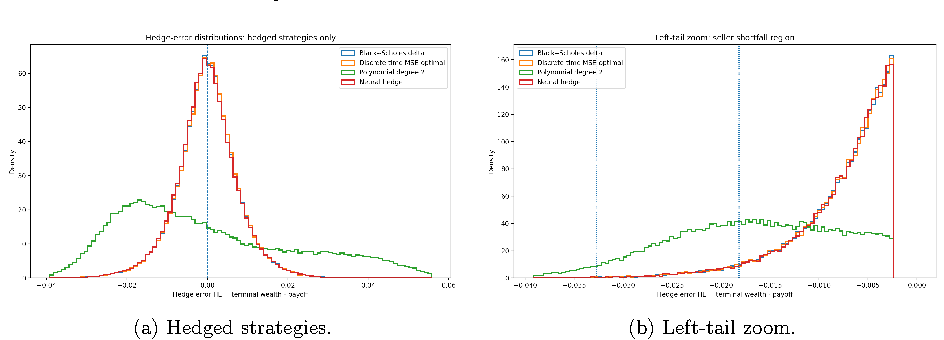
\includegraphics[width=0.98\textwidth,height=4.65cm,keepaspectratio]
    {figures/report_fig_3_2_hedge_error_distributions.pdf}

  \vspace{0.08cm}
  \academicbox[0.94\textwidth]{\centering\small
    The neural residual-error distribution closely matches the two analytic hedges,
    including in the seller-shortfall tail.}
  \vspace{0.06cm}
  {\scriptsize\color{Slate}\bfseries
    Analytic overlap across the full distribution\quad\textcolor{Teal}{|}\quad
    polynomial hedge materially wider\par}
  \sourcefoot{Submitted report, Figure 3.2 and Sec.\ 3.1.4. Tight vector crop from final report PDF p.\ 20 (printed p.\ 16).}
  \note{Start with the full distribution, then point to the seller-shortfall zoom. The neural, Black--Scholes and discrete-time curves nearly overlap, while the polynomial distribution is visibly wider. This is distributional confirmation, not only one RMSE number.}
\end{frame}

\speakerlabel{Siphelele}{1:40}
\begin{frame}[t]{\texorpdfstring{\resizebox{0.94\textwidth}{!}{Why crude Monte Carlo was sufficient at the final path budget}}{Why crude Monte Carlo was sufficient at the final path budget}}
  \centering
  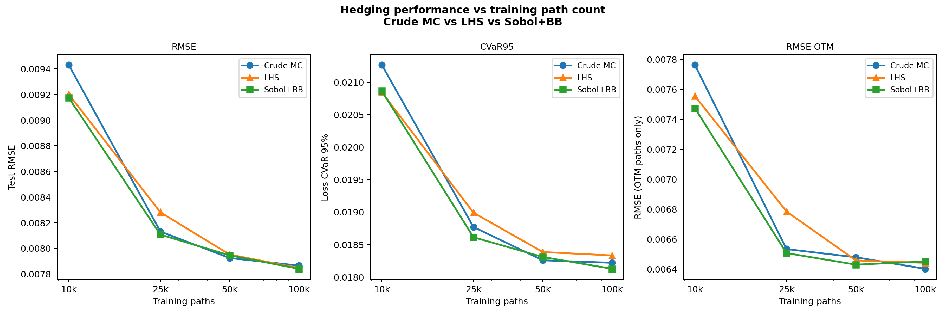
\includegraphics[width=0.98\textwidth,height=3.55cm,keepaspectratio]
    {figures/report_fig_A_1_sampling_path_count.pdf}

  \vspace{0.08cm}
  \begin{columns}[T,onlytextwidth]
    \begin{column}{0.31\textwidth}
      \academicbox{\centering
        {\color{Coral}\large\bfseries 10k paths\par}
        {\scriptsize structured sampling improves RMSE by roughly 2--3\%, especially OTM}}
    \end{column}
    \begin{column}{0.31\textwidth}
      \academicbox{\centering
        {\color{Gold!80!black}\large\bfseries 50k paths\par}
        {\scriptsize differences are already negligible}}
    \end{column}
    \begin{column}{0.31\textwidth}
      \academicbox{\centering
        {\color{Teal}\large\bfseries 100k paths\par}
        {\scriptsize no material performance difference}}
    \end{column}
  \end{columns}
  \vspace{0.08cm}
  \claimbox{Crude Monte Carlo retained at the final training scale.}
  \vspace{0.03cm}
  {\scriptsize\color{DeepNavy}\bfseries
    The controlled benchmark is recovered, and the conclusion is stable at the final data budget.\par}
  \sourcefoot{Submitted report, Figure A.1, Table A.8 and Sec.\ 3.1.5. Tight vector crop from final report PDF p.\ 48 (printed p.\ 44).}
  \note{Structured sampling helped at low path budgets, with the clearest advantage in the OTM panel. By 50,000 paths the curves have essentially converged, and at 100,000 paths the advantage disappeared. Use the closing line to hand directly to Micaela.}
\end{frame}
